\documentclass[journal,12pt,twocolumn]{IEEEtran}

\usepackage{setspace}
\usepackage{gensymb}

\singlespacing


\usepackage[cmex10]{amsmath}

\usepackage{amsthm}

\usepackage{mathrsfs}
\usepackage{txfonts}
\usepackage{stfloats}
\usepackage{bm}
\usepackage{cite}
\usepackage{cases}
\usepackage{subfig}

\usepackage{longtable}
\usepackage{multirow}

\usepackage{enumitem}
\usepackage{mathtools}
\usepackage{steinmetz}
\usepackage{tikz}
\usepackage{circuitikz}
\usepackage{verbatim}
\usepackage{tfrupee}
\usepackage[breaklinks=true]{hyperref}
\usepackage{graphicx}
\usepackage{tkz-euclide}

\usetikzlibrary{calc,math}
\usepackage{listings}
    \usepackage{color}                                            %%
    \usepackage{array}                                            %%
    \usepackage{longtable}                                        %%
    \usepackage{calc}                                             %%
    \usepackage{multirow}                                         %%
    \usepackage{hhline}                                           %%
    \usepackage{ifthen}                                           %%
    \usepackage{lscape}     
\usepackage{multicol}
\usepackage{chngcntr}

\DeclareMathOperator*{\Res}{Res}

\renewcommand\thesection{\arabic{section}}
\renewcommand\thesubsection{\thesection.\arabic{subsection}}
\renewcommand\thesubsubsection{\thesubsection.\arabic{subsubsection}}

\renewcommand\thesectiondis{\arabic{section}}
\renewcommand\thesubsectiondis{\thesectiondis.\arabic{subsection}}
\renewcommand\thesubsubsectiondis{\thesubsectiondis.\arabic{subsubsection}}


\hyphenation{op-tical net-works semi-conduc-tor}
\def\inputGnumericTable{}                                 %%

\lstset{
%language=C,
frame=single, 
breaklines=true,
columns=fullflexible
}
\begin{document}


\newtheorem{theorem}{Theorem}[section]
\newtheorem{problem}{Problem}
\newtheorem{proposition}{Proposition}[section]
\newtheorem{lemma}{Lemma}[section]
\newtheorem{corollary}[theorem]{Corollary}
\newtheorem{example}{Example}[section]
\newtheorem{definition}[problem]{Definition}

\newcommand{\BEQA}{\begin{eqnarray}}
\newcommand{\EEQA}{\end{eqnarray}}
\newcommand{\define}{\stackrel{\triangle}{=}}
\bibliographystyle{IEEEtran}
\providecommand{\mbf}{\mathbf}
\providecommand{\pr}[1]{\ensuremath{\Pr\left(#1\right)}}
\providecommand{\qfunc}[1]{\ensuremath{Q\left(#1\right)}}
\providecommand{\sbrak}[1]{\ensuremath{{}\left[#1\right]}}
\providecommand{\lsbrak}[1]{\ensuremath{{}\left[#1\right.}}
\providecommand{\rsbrak}[1]{\ensuremath{{}\left.#1\right]}}
\providecommand{\brak}[1]{\ensuremath{\left(#1\right)}}
\providecommand{\lbrak}[1]{\ensuremath{\left(#1\right.}}
\providecommand{\rbrak}[1]{\ensuremath{\left.#1\right)}}
\providecommand{\cbrak}[1]{\ensuremath{\left\{#1\right\}}}
\providecommand{\lcbrak}[1]{\ensuremath{\left\{#1\right.}}
\providecommand{\rcbrak}[1]{\ensuremath{\left.#1\right\}}}
\theoremstyle{remark}
\newtheorem{rem}{Remark}
\newcommand{\sgn}{\mathop{\mathrm{sgn}}}
\providecommand{\abs}[1]{\vert#1\vert}
\providecommand{\res}[1]{\Res\displaylimits_{#1}} 
\providecommand{\norm}[1]{\Vert#1\rVert}
%\providecommand{\norm}[1]{\lVert#1\rVert}
\providecommand{\mtx}[1]{\mathbf{#1}}
\providecommand{\mean}[1]{E[ #1 ]}
\providecommand{\fourier}{\overset{\mathcal{F}}{ \rightleftharpoons}}
%\providecommand{\hilbert}{\overset{\mathcal{H}}{ \rightleftharpoons}}
\providecommand{\system}{\overset{\mathcal{H}}{ \longleftrightarrow}}
	%\newcommand{\solution}[2]{\textbf{Solution:}{#1}}
\newcommand{\solution}{\noindent \textbf{Solution: }}
\newcommand{\cosec}{\,\text{cosec}\,}
\providecommand{\dec}[2]{\ensuremath{\overset{#1}{\underset{#2}{\gtrless}}}}
\newcommand{\myvec}[1]{\ensuremath{\begin{pmatrix}#1\end{pmatrix}}}
\newcommand{\mydet}[1]{\ensuremath{\begin{vmatrix}#1\end{vmatrix}}}
\numberwithin{equation}{subsection}
\makeatletter
\@addtoreset{figure}{problem}
\makeatother
\let\StandardTheFigure\thefigure
\let\vec\mathbf
\renewcommand{\thefigure}{\theproblem}
\def\putbox#1#2#3{\makebox[0in][l]{\makebox[#1][l]{}\raisebox{\baselineskip}[0in][0in]{\raisebox{#2}[0in][0in]{#3}}}}
     \def\rightbox#1{\makebox[0in][r]{#1}}
     \def\centbox#1{\makebox[0in]{#1}}
     \def\topbox#1{\raisebox{-\baselineskip}[0in][0in]{#1}}
     \def\midbox#1{\raisebox{-0.5\baselineskip}[0in][0in]{#1}}
\vspace{3cm}
\title{ASSIGNMENT-2}
\author{B.ANUSHA}
\maketitle
\newpage
\bigskip
\renewcommand{\thefigure}{\theenumi}
\renewcommand{\thetable}{\theenumi}
Download all python codes from 
\begin{lstlisting}
https://github.com/BOJJAVOYINAANUSHA/Assignment-2/blob/main/ASSIGNMENT2/assignment2.py
\end{lstlisting}
%
and latex-tikz codes from 
%
\begin{lstlisting}
https://github.com/BOJJAVOYINAANUSHA/Assignment-2/blob/main/ASSIGNMENT2/main.tex
\end{lstlisting}
%
\section{Question No. 2.42}
Construct ABCD where $AB = 4, BC = 5, CD = 6.5, \angle B = 105 \degree$ and $\angle C = 80 \degree$.
%
\section{SOLUTION}
\begin{enumerate}
\item Let us assume vertices of given quadrilateral $ABCD$ as $\vec{A}$,$\vec{B}$,$\vec{C}$ and $\vec{D}$.
\item Let us generalize the given data:
    \begin{align}
    &\angle B= 105\degree=\theta \label{eq1}
    \\
    &\angle C= 80\degree=\alpha \label{eq2}
    \\
    &\norm{\vec{A}-\vec{B}} =4=p \label{eq3}
    \\
    &\norm{\vec{C}-\vec{B}} =5=q \label{eq4}
    \\
     &\norm{\vec{D}-\vec{C}} =6.5=r \label{eq5}
    \end{align}
\begin{itemize}
\item For this quadrilateral $ABCD$ we have,
\begin{align}
\angle B +\angle C = 105\degree + 80\degree =185\degree
\end{align}
\item Let, \begin{align}
    &\vec{B}=\myvec{0\\0}, \vec{C}=\myvec{5\\0} \label{eq6}
\end{align}
\end{itemize}
\begin{lemma}
\label{lemma}
The coordinate of \textbf{A} and \textbf{D} can be written as follows:
\begin{align}
\implies \vec{A}= p \myvec{\cos B \\\sin B } \label{eq a}
\\
\implies \vec{D}=\myvec{5\\0} + r \myvec{\cos C\\\sin C } \label{eq b}
\end{align}
\end{lemma}
\item For finding coordinates of A:-
\\
The vector equation of line is given by:
\begin{align}
\vec{A}=\vec{B} + p \vec{b} 
\end{align}
\ putting \eqref{eq1} and \eqref{eq3} in \eqref{eq a} we get,
\begin{align}
&\implies \vec{A}=4\myvec{\cos 105 \\\sin 105 }
\\
&\implies \vec{A}=\myvec{-1.03\\3.86}
\end{align}
\item For finding coordinates of D:-
\\
The vector equation of line is given by:
\begin{align}
\vec{D}=\vec{C} + r \vec{c}
\end{align}
\ Putting \eqref{eq2} and \eqref{eq5} in \eqref{eq b} we get,
\begin{align}
&\implies \vec{D}=\myvec{5\\0} + 6.5\myvec{\cos 80 \\\sin 80 }
\\
&\implies \vec{D}=\myvec{5\\0} + \myvec{1.12\\6.39}
\\
&\implies \vec{D}=\myvec{6.12\\6.39}
\end{align}
\begin{itemize}
\item Now,the vertices of given Quadrilateral ABCD can be written as,
\end{itemize}
\begin{align}
 \vec{A}=\myvec{-1.03\\3.86},\vec{B} = \myvec{0\\0}, \vec{C}=\myvec{5\\0},\vec{D}=\myvec{6.12\\6.39}
\end{align}
    \item On constructing the quadrilateral $ABCD$ we get:
\end{enumerate}   
\numberwithin{figure}{section}
\begin{figure}[!ht]
\centering
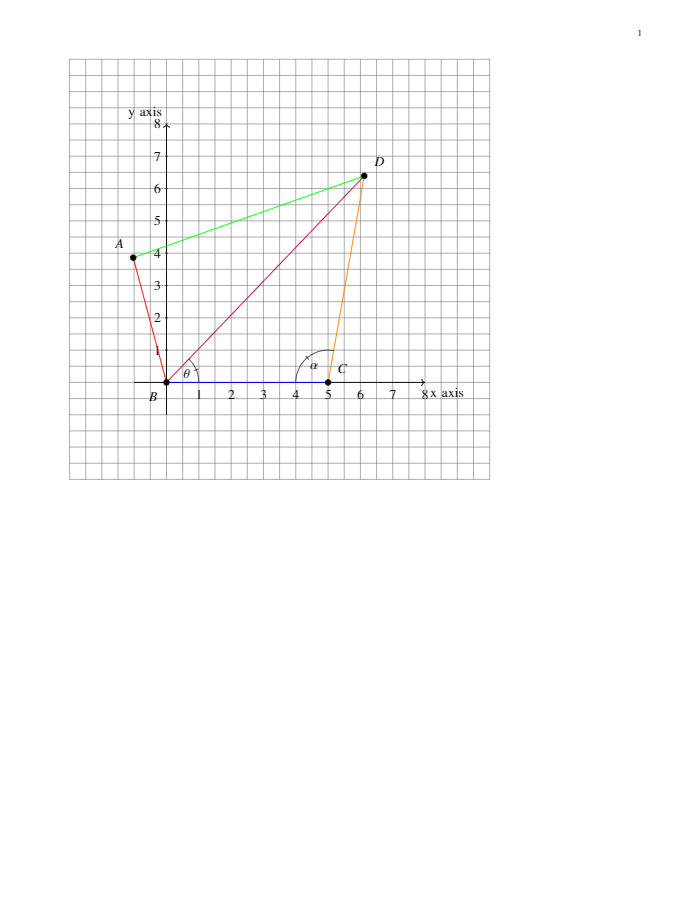
\includegraphics[ width=\columnwidth ,height= 16cm]{FIGURE.png}
\caption{Quadrilateral ABCD}
\label{fig:Quadrilateral ABCD}	
\end{figure}
\end{document}
